\chapter{Makerchip-NgVeri: Mixed Signal Simulation}
\label{chap10}
\thispagestyle{empty}

NgVeri is a simulator in eSim which facilitates mixed-signal circuit simulation. Digital models are simulated using Verilator and analog models are simulated using XSPICE engine of Ngspice. NgVeri links Ngspice and Verilator to support mixed-mode simulations in eSim as shown in \figref{ngveriblock}. 


\begin{figure}[H]
\centering
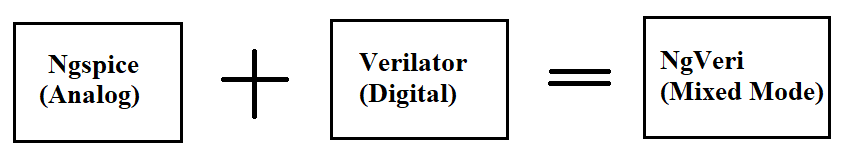
\includegraphics[ height = 2cm]{./NgVeri/ngveri_block.png}
\caption{NgVeri Block}
\label{ngveriblock}
\end{figure}

 
\noindent {Makerchip is a web browser IDE to develop/simulate/debug Verilog, SystemVerilog and TL-Verilog Code developed by Redwood EDA, LLC. It provides seamless design experience by integrating code, debug window, block diagrams, waveforms together in one screen. Makerchip is integrated with NgVeri in the latest version of eSim (eSim 2.2). Makerchip provides the digital side of eSim's mixed-signal environment.} 


\section{Familiarizing the Makerchip-NgVeri interface in eSim}

In this section, we will explain Makerchip-NgVeri interface in eSim and the various menus and tabs.
 
\begin{figure}[H]
\centering
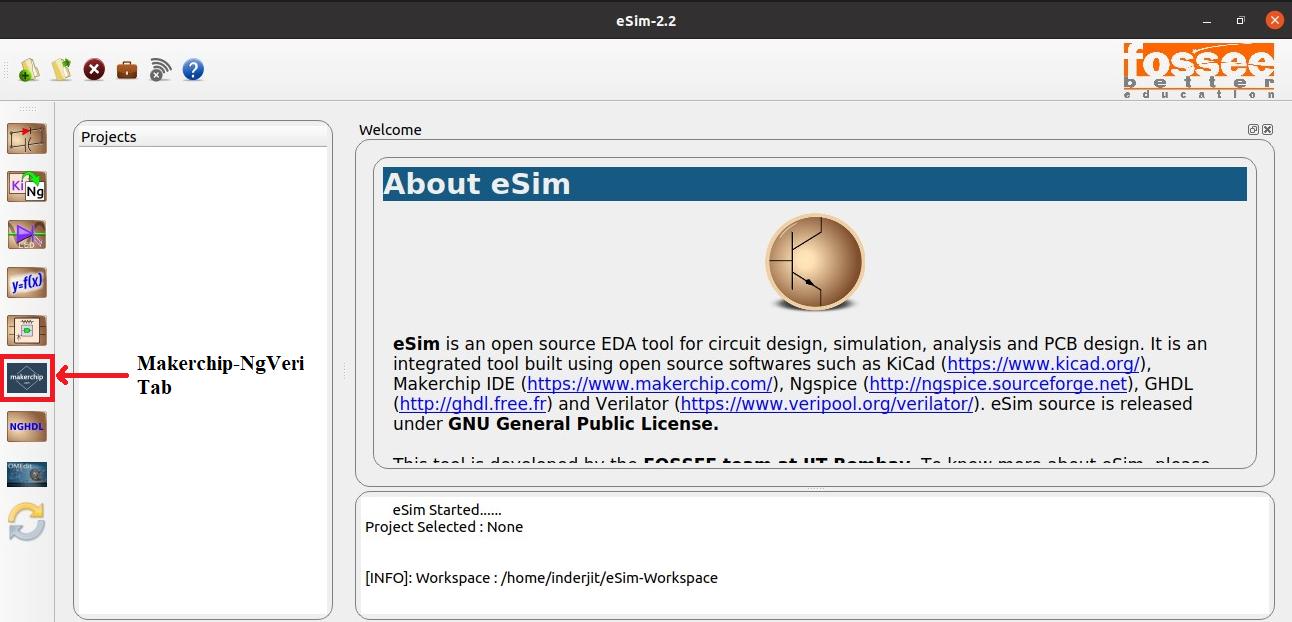
\includegraphics[width = 14cm, height = 7cm]{./NgVeri/MakerchipNgVeriicon.png}
\caption{Makerchip NgVeri Tab}
\label{makerchipngveri}
\end{figure}

%description of makerchip:
\figref{makerchipngveri} shows the Makerchip-NgVeri tab (newly added in eSim 2.2). In order to open this tab click on the Makerchip button on LHS vertical bar. Makerchip interface opens up as shown in the \figref{makerchipinterface}. 

\begin{figure}[H]
\centering
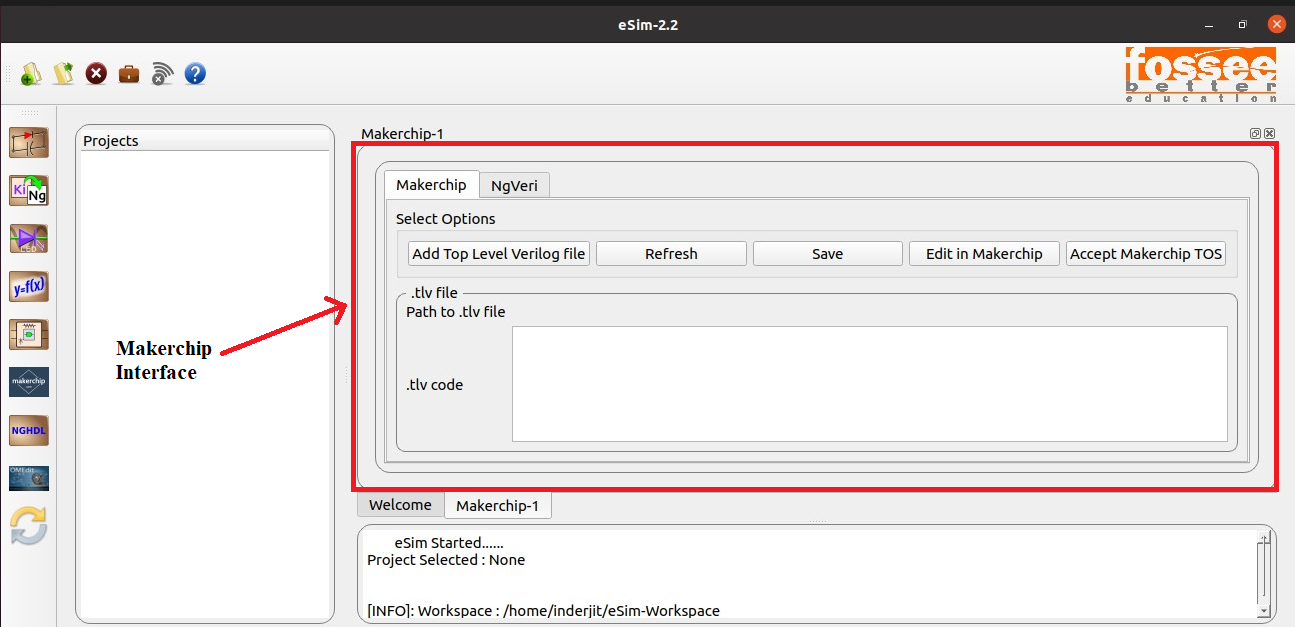
\includegraphics[width = 14cm, height = 7cm]{./NgVeri/makerchipinterface.png}
\caption{Makerchip Interface}
\label{makerchipinterface}
\end{figure}

\pagebreak

\section{Makerchip Interface}

%Description of Makerchip interface
Makerchip interface working space is shown in the \figref{makerchipinterface}. Various buttons of Makerchip interface are shown in the \figref{makerchipbuttons}

\begin{figure}[H]
\centering
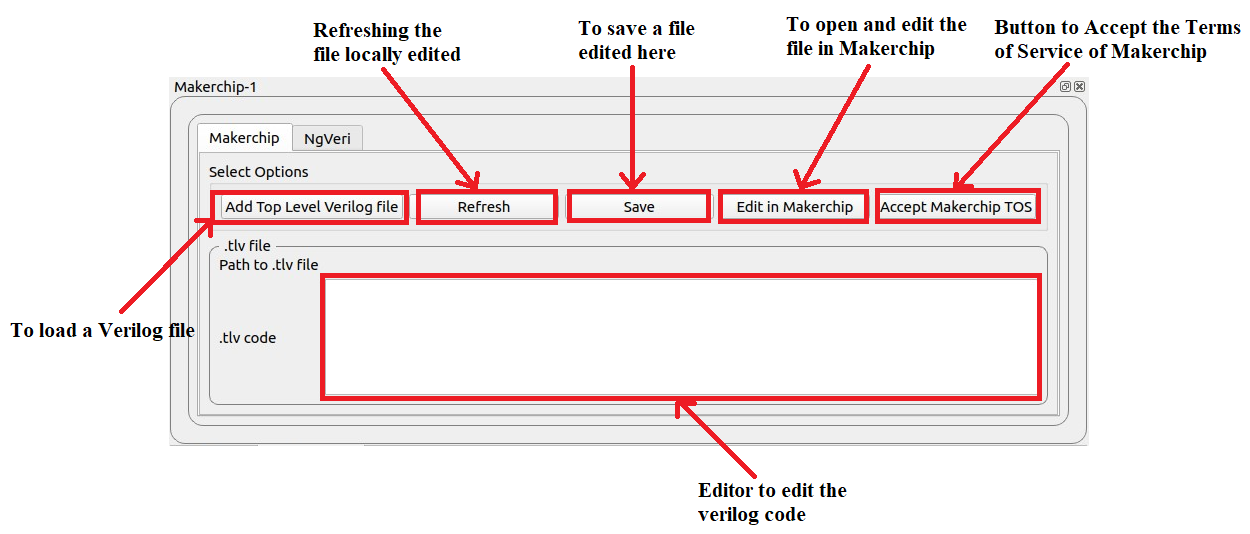
\includegraphics[width = 14cm, height = 7cm]{./NgVeri/makerchipbuttons.png}
\caption{Makerchip buttons}
\label{makerchipbuttons}
\end{figure}

\noindent \textbf{The components of the Makerchip tab are}:

\begin{enumerate}
\item Add Top Level Verilog file: This button helps the user to load the verilog file. 

\item Refresh: It enables refreshing of the file locally edited. 

\item Save: It saves the edited file. 

\item Edit in Makerchip: It opens the Makerchip App and the user can edit and simulate the verilog file in Makerchip IDE.

\item .tlv Code Editor: After loading the top level verilog file, the verilog code appears in this editor. The user can then edit the verilog code within this editor workspace. 

\item Path to .tlv file: The path or the directory where the verilog file exists locally appears here after uploading the verilog file.

\item Accept Makerchip TOS: This button when pressed accepts the Terms of Service of Makerchip. After accepting this, the button vanishes in the rerun of eSim. 

\end{enumerate}

\pagebreak

\section{NgVeri Interface}

%Description of Makerchip interface
NgVeri interface is shown in the \figref{ngveriinterface}. Various components of NgVeri interface are shown in the \figref{ngveributtons}

\begin{figure}[!htp]
\centering
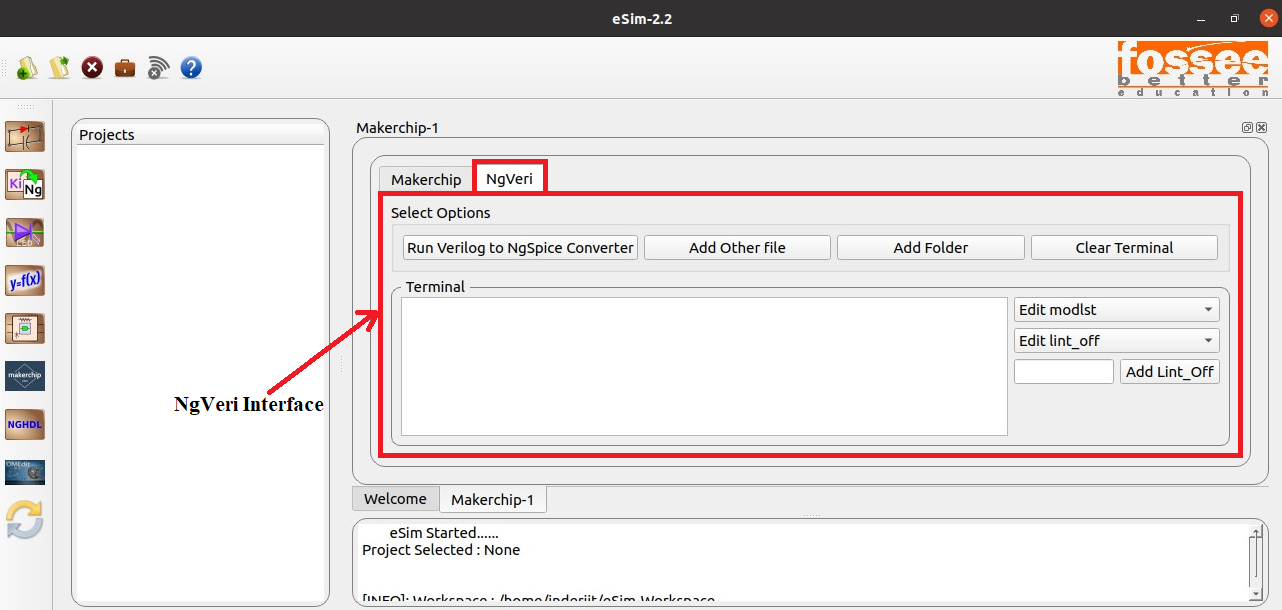
\includegraphics[width = 13cm, height = 7cm]{./NgVeri/ngveriinterface.png}
\caption{NgVeri Interface}
\label{ngveriinterface}
\end{figure}


\noindent \textbf{The important components of NgVeri are:}

\begin{enumerate}

\item Terminal : This is the terminal where the user can view all the commands and processes running. 

\item Run Verilog to Ngspice Converter: This button when pressed run NgVeri and builds the model for Ngspice. 

\item Add Other file: Using this option, the user can add all the dependency files which are needed by the Top level verilog file in Makerchip.

\item Add Folder: Using this option, the user can add all the dependency folders which are needed by the Top level verilog file.

\item Clear terminal: This button when pressed erases the content of the terminal i.e it clears the terminal.

\item Edit modlst: Using this option, the user can see the existing models present and the user can remove the models from the Model list. 

\begin{figure}[H]
\centering
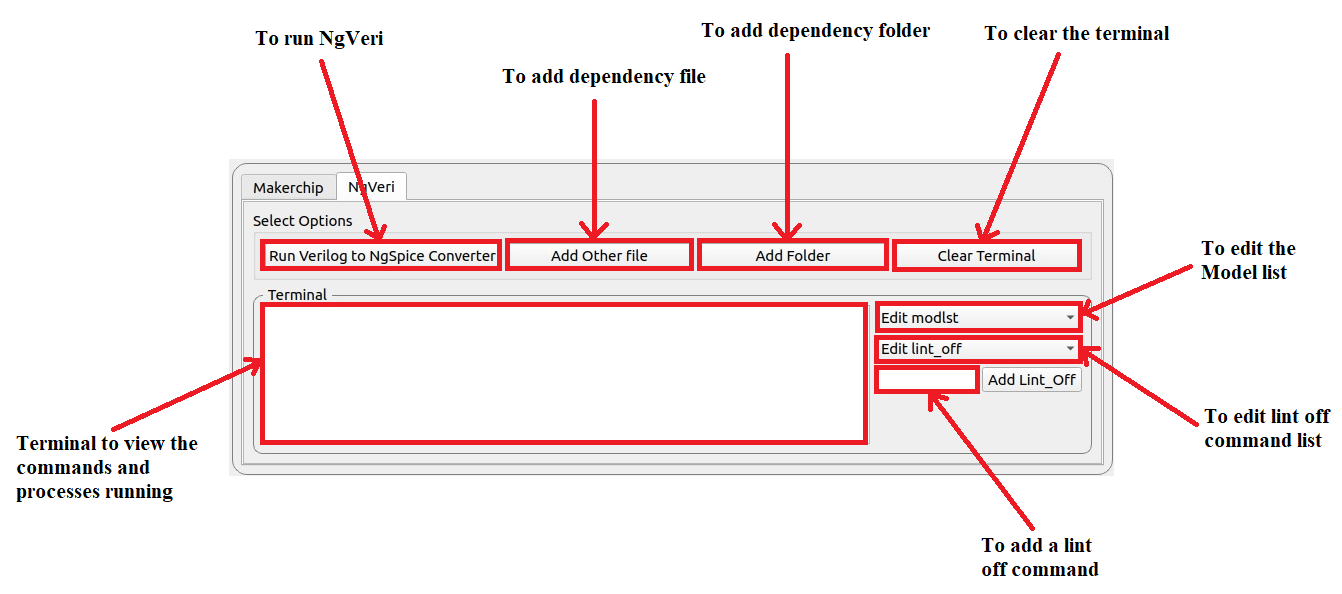
\includegraphics[width = 15cm, height = 8cm]{./NgVeri/ngveributtons.png}
\caption{NgVeri buttons}
\label{ngveributtons}
\end{figure}

\item Edit lint off:  When this button is pressed, the user can see all the lint-off commands list and the user can remove the lint-off from the list. 

\item Add Lint off: The user can add lint-off command by using this button. This lint-off command is used if user gets a lint-off error in the terminal.

\end{enumerate}

\newpage

\section{Counter example using Makerchip and NgVeri in eSim}

%Description of Sample schematic creation
In this section, a digital 8 bit counter example using NgVeri and Makerchip tabs in eSim is discussed. Kindly note that steps shown over here are carried out with eSim 2.2 in Ubuntu version 20.04. Steps remain same for eSim in Windows version.


\subsection {Makerchip steps in eSim}

Steps for verilog code compilation and verification using Makerchip IDE are as follows: 

\begin{enumerate}

\item Open eSim and select the default eSim workspace by clicking on \textbf{OK} as shown in \figref{workspaceeSim}. Its format is /home/$<$username$>$/eSim-Workspace. User-name can be user specific but be careful of the naming conventions(space is not allowed). If the user wants to select they can chose the same by using the \textbf{Browse} button in the dialog box.

\begin{figure}[H]
\centering
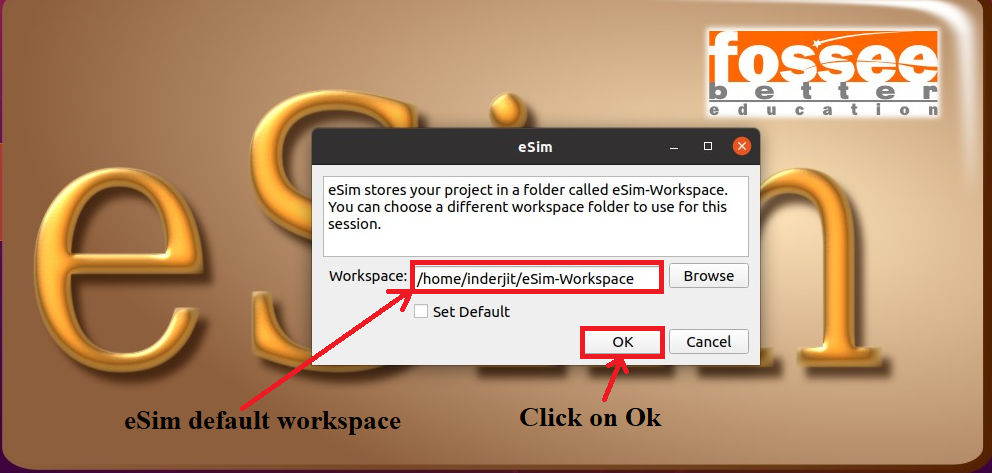
\includegraphics[width = 9cm, height = 5cm]{./NgVeri/defaultworkspace.png}
\caption{eSim workspace}
\label{workspaceeSim}
\end{figure}

\item Open a blank Text Editor and write verilog code of 8 bit counter and save the file as either filename.v in the eSim-Workspace as shown in \figref{savingv}. 
\item \textbf{Please Note}: The filename should be the same as top-level module name, otherwise eSim will throw an error as discussed in Common error sections.\\
The file extensions allowed are:
\begin{itemize}
    \item .v for Verilog 
    \item .sv for SystemVerilog
    \item .tlv for Transaction-Level Verilog
\end{itemize}

\begin{figure}[H]
\centering
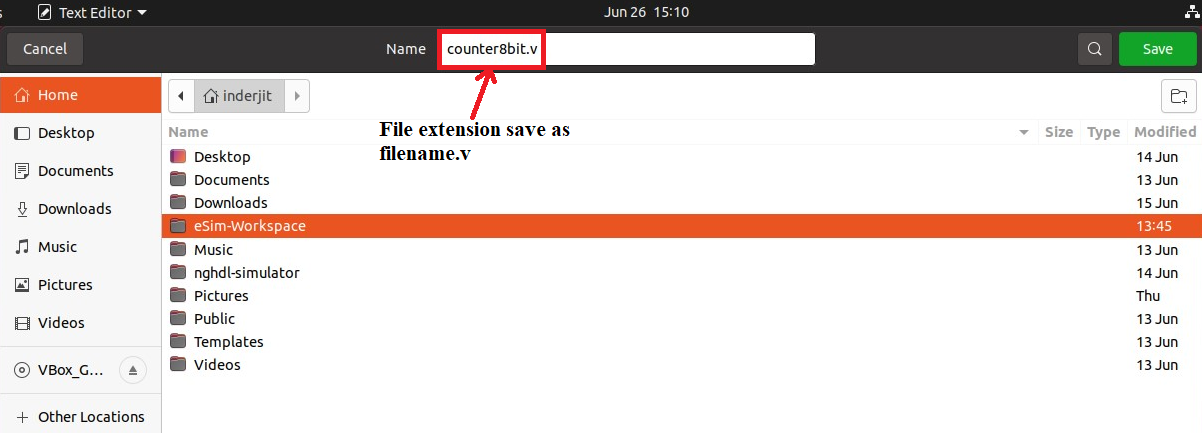
\includegraphics[width = 14cm, height = 5cm]{./NgVeri/savingvfile.png}
\caption{Saving verilog file in eSim workspace}
\label{savingv}
\end{figure}

\item The verilog code for 8 bit counter is written inside the Text Editor with .v file as extension saved in eSim workspace is shown in \figref{vcode}

\begin{figure}[H]
\centering
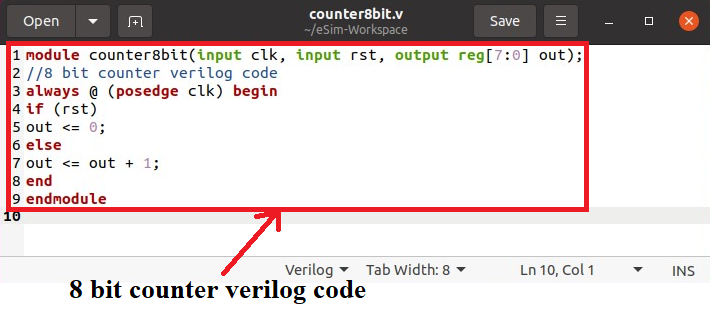
\includegraphics[width = 11cm, height = 5cm]{./NgVeri/verilogcode.png}
\caption{8 bit Counter verilog code}
\label{vcode}
\end{figure}

\item Click on Makerchip-NgVeri button on the left toolbar of eSim window which opens Makerchip interface in eSim as shown in \figref{addingv}. 

\begin{figure}[H]
\centering
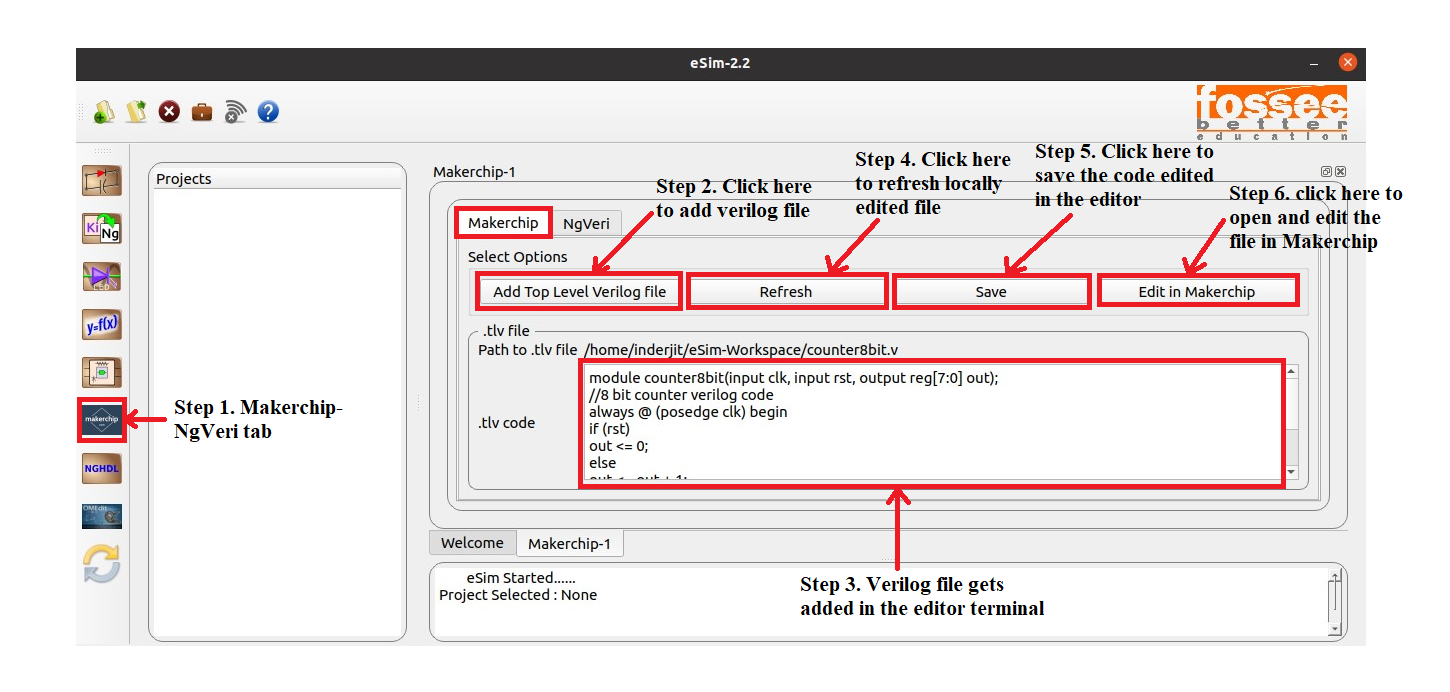
\includegraphics[width = 15cm, height =7cm]{./NgVeri/addingvfile.png}
\caption{Adding verilog file in Makerchip editor}
\label{addingv}
\end{figure}

\item Click on the button shown in Step 2 as shown in \figref{addingv} to add the verilog file for 8 bit counter. The path to top level verilog file along with the verilog code get added in the Makerchip editor terminal shown in Step 3 of \figref{addingv}

\item User can refresh locally edited verilog file by clicking on the \textbf{Refresh} button as shown in Step 4 of \figref{addingv}. If the file is edited using some other editor and also loaded in Makerchip Tab at the same time, the \textbf{Refresh} button starts toggling. The user must click on the Refresh button to get the new version of the file in the editor.

\item User can save the verilog code edited in the Makerchip editor terminal by clicking on the \textbf{Save} button shown in Step 5 of \figref{addingv}

\item For the first run, the user needs to accept the Term of Service by clicking on \textbf{Accept Makerchip TOS} as shown in \figref{TOS}. This button will disappear after rerun of eSim as shown in \figref{addingv}. 

\begin{figure}[H]
\centering
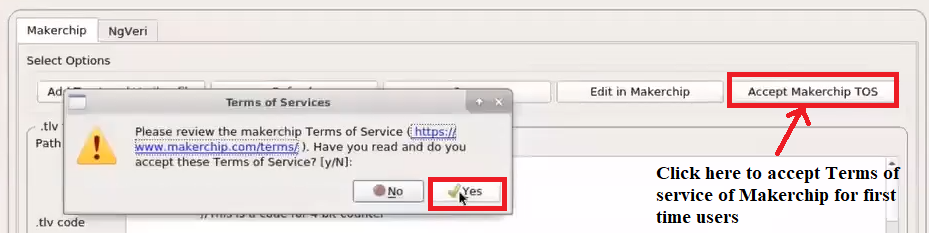
\includegraphics[width = 13cm, height = 4cm]{./NgVeri/acceptTOS.png}
\caption{Accepting Terms of Service of Makerchip}
\label{TOS}
\end{figure}

\item Now click on \textbf{Edit in Makerchip} button to open and edit the verilog code in Makerchip IDE. A pop-up window will appear as shown in \figref{editinmakerchip}. By clicking on \textbf{Yes}, a top level verilog file i.e .tlv file will be created in the same directory of current verilog file and the Makerchip IDE will be run in a new web browser as shown in \figref{makerchipide}. By clicking on \textbf{No}, the current raw verilog file i.e .v file will open up in Makerchip IDE web browser. 

\begin{figure}[H]
\centering
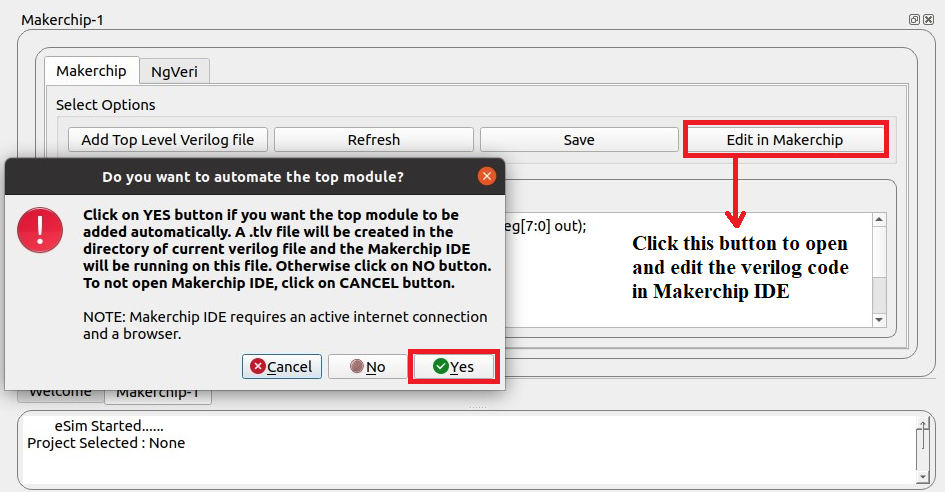
\includegraphics[width = 14cm, height = 6cm]{./NgVeri/editinmakerchip.png}
\caption{Opening Makerchip IDE}
\label{editinmakerchip}
\end{figure}

\begin{figure}[H]
\centering
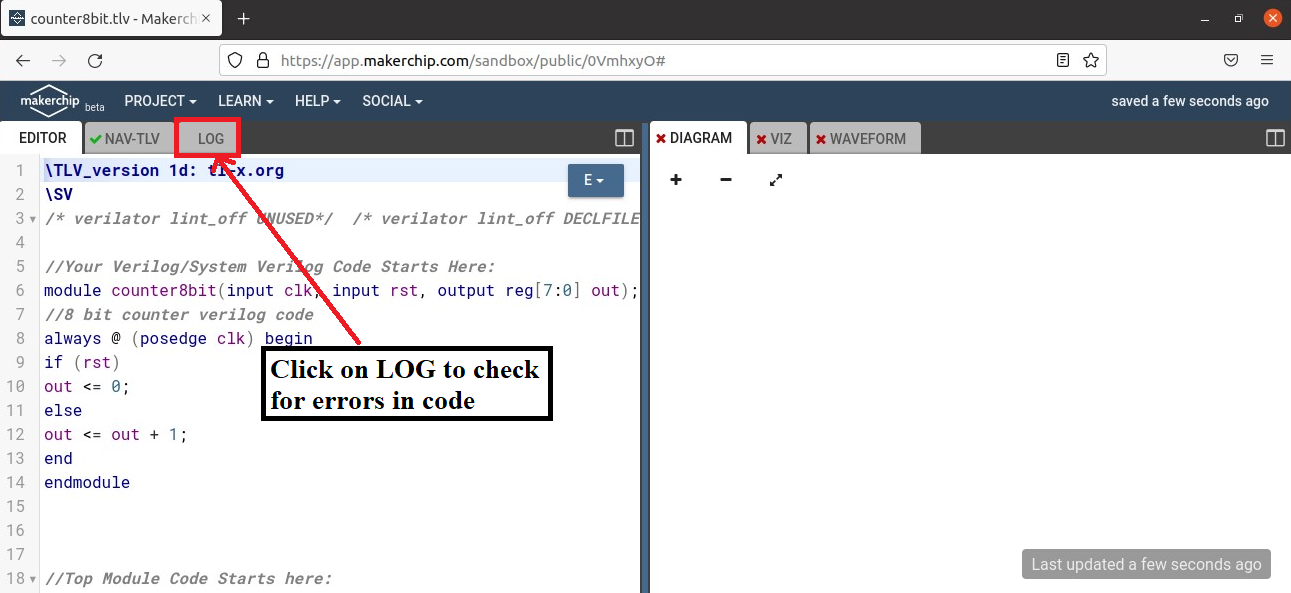
\includegraphics[width = 14cm, height = 6cm]{./NgVeri/makerchipIDE.png}
\caption{Makerchip IDE interface}
\label{makerchipide}
\end{figure}

\item User can check for errors by clicking on \textbf{LOG} tab in Makerchip IDE interface as shown in the \figref{makerchipide}. Following window will appear as shown in \figref{makerchiperror}, where you can check the Verilator lint-off errors. 

\begin{figure}[H]
\centering
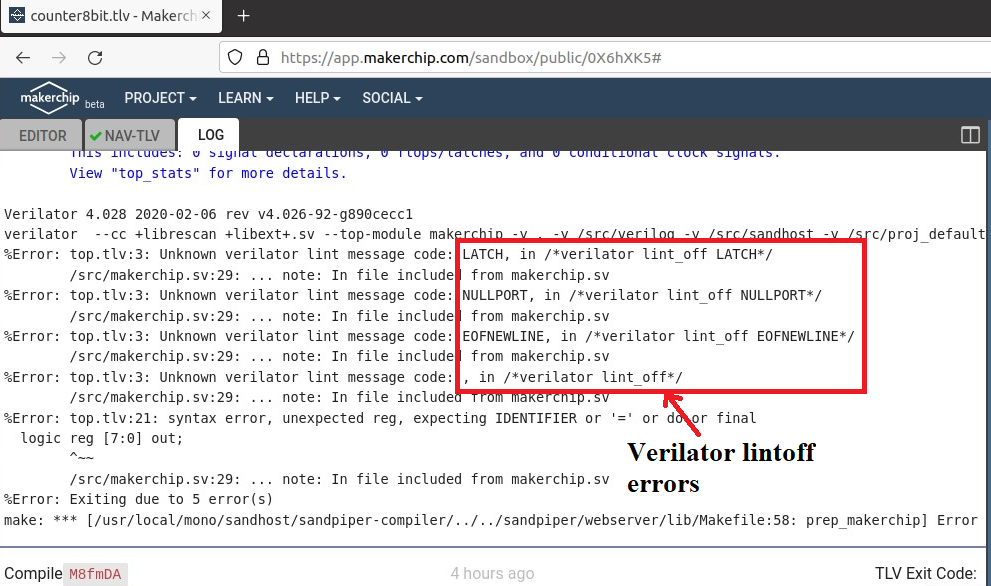
\includegraphics[width = 14cm, height =7cm]{./NgVeri/makerchiperrors.png}
\caption{Verilator lintoff errors}
\label{makerchiperror}
\end{figure}

\item As shown in the \figref{makerchiperror}, verilator lint-off commands which caused error in the Log section needs to be removed from Line 3 in the editor window. Two such commands which needs to be removed are shown in the \figref{lintofferror}.

\begin{figure}[H]
\centering
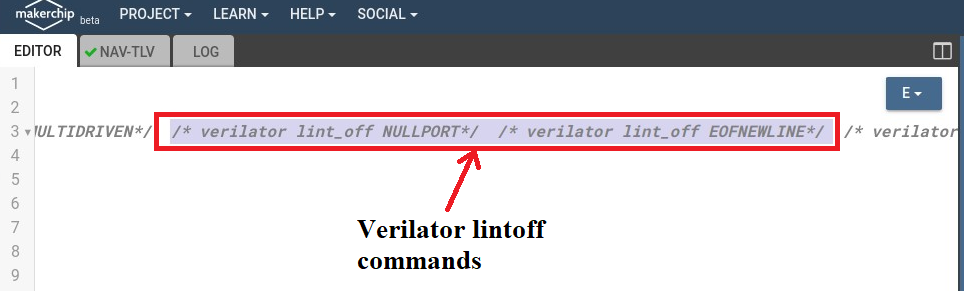
\includegraphics[width = 12cm, height =4cm]{./NgVeri/lintofferror.png}
\caption{Removal of lintoff errors}
\label{lintofferror}
\end{figure}

\item Next, click on the \textbf{Editor} tab in the editor as shown in \figref{compile1}, then click on \textbf{Compile/Sim} button to compile the verilog code. 

\begin{figure}[H]
\centering
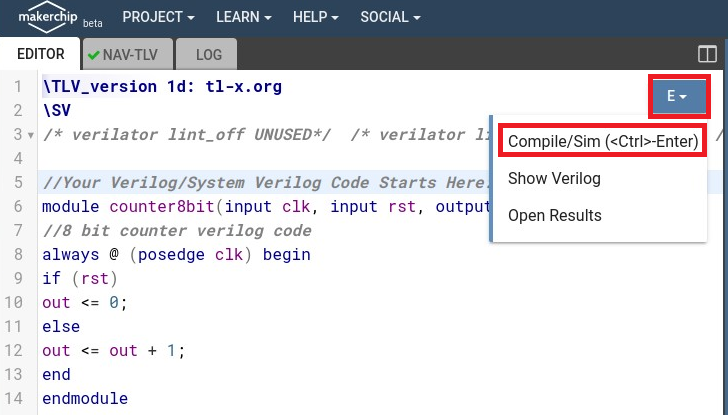
\includegraphics[width = 12cm, height =5cm]{./NgVeri/compile1.png}
\caption{Compiling after removing lintoff errors}
\label{compile1}
\end{figure}

\begin{figure}[H]
\centering
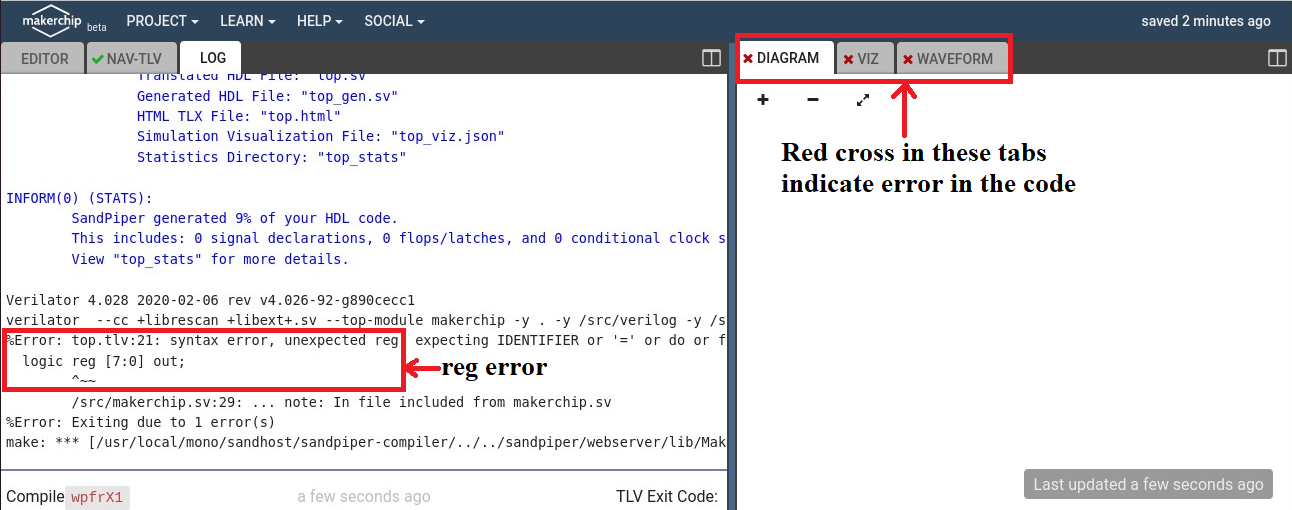
\includegraphics[width = 14cm, height =6cm]{./NgVeri/regerror.png}
\caption{ Unexpected reg error in the code}
\label{regerror}
\end{figure}

\item After compiling, \textbf{Unexpected reg error} remains in the Log section (Refer \figref{regerror}) which can be rectified by removing \textit{reg} from top level verilog code as shown in \figref{removereg}. By clicking \textbf{Yes} button in \figref{editinmakerchip}, a Top Level Verilog (TLV) code automatically gets added in the editor. Refer \figref{removereg}. The value of \textit{rst} value is by default as random value and it can be replaced if user wants to assign values. We have assigned \textit{rst} with \textit{reset} in this counter example. 

\begin{figure}[H]
\centering
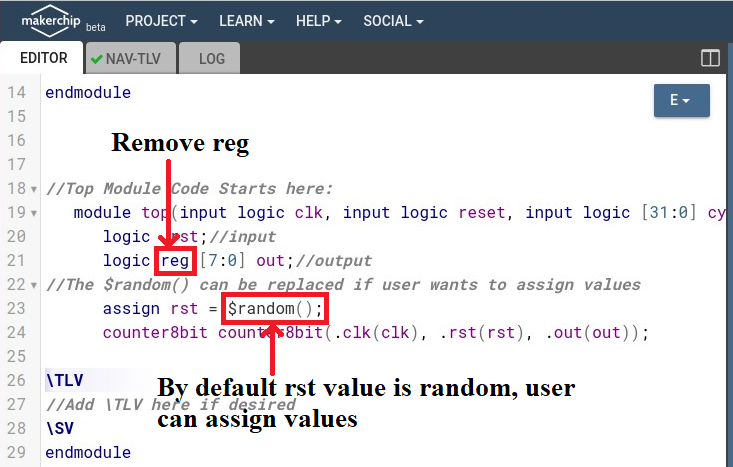
\includegraphics[width = 12cm, height =6cm]{./NgVeri/removereg.png}
\caption{Top level verilog code}
\label{removereg}
\end{figure}

\item Now click on the \textbf{Editor} tab and then click on \textbf{Compile/Sim} button in the editor as shown in \figref{compile1}, it will display the following waveform window as shown in \figref{output1}. This means that the verilog code of 8 bit Counter is successfully compiled. Kindly, note that in \figref{output1}, inputs and output waveform are in the compressed form. 

\begin{figure}[H]
\centering
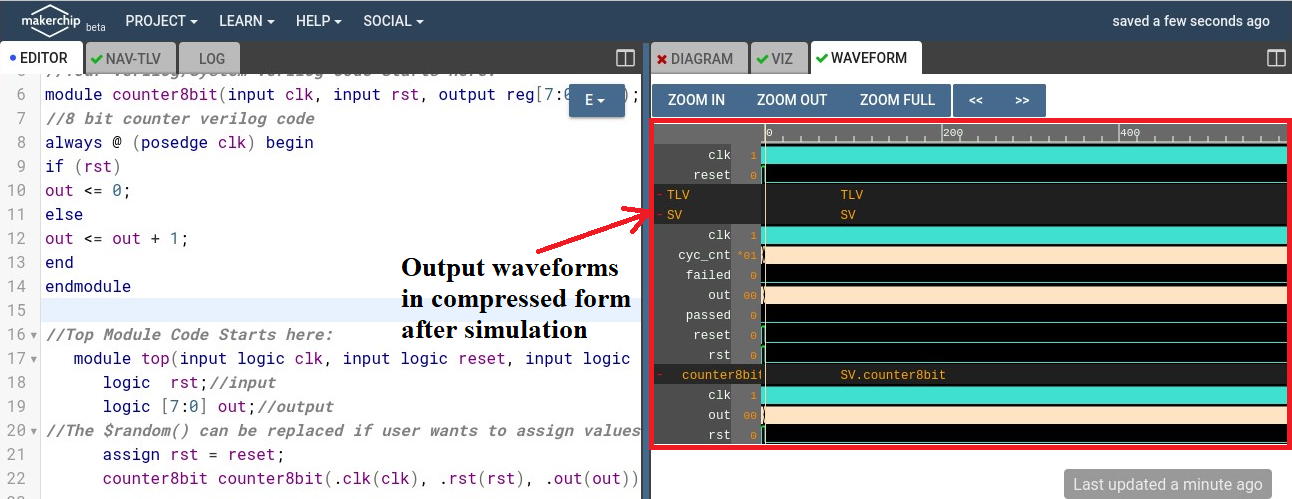
\includegraphics[width = 14cm, height =6cm]{./NgVeri/makerchipoutput1.png}
\caption{Output waveforms in compressed form of 8 bit Counter }
\label{output1}
\end{figure}

\item \figref{output2} shows the expanded view of inputs and output waveforms of 8 bit counter. The waveforms in \figref{output1} can be expanded by clicking on \textbf{Zoom In} button as shown in \figref{output2}.

\begin{figure}[H]
\centering
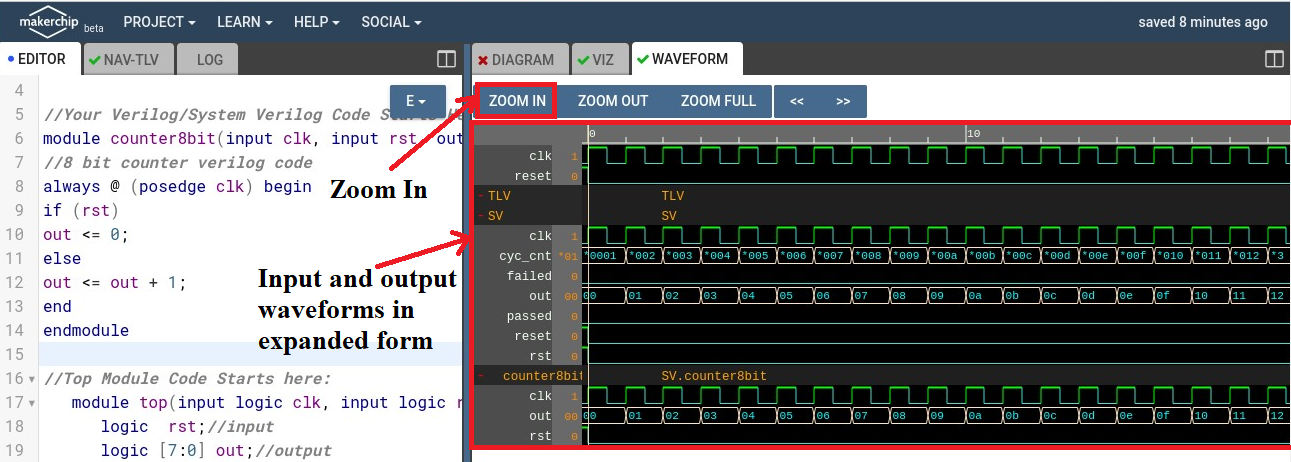
\includegraphics[width = 14cm, height =6cm]{./NgVeri/makerchipoutput2.png}
\caption{Output waveforms in expanded form of 8 bit Counter }
\label{output2}
\end{figure}

\begin{figure}[H]
\centering
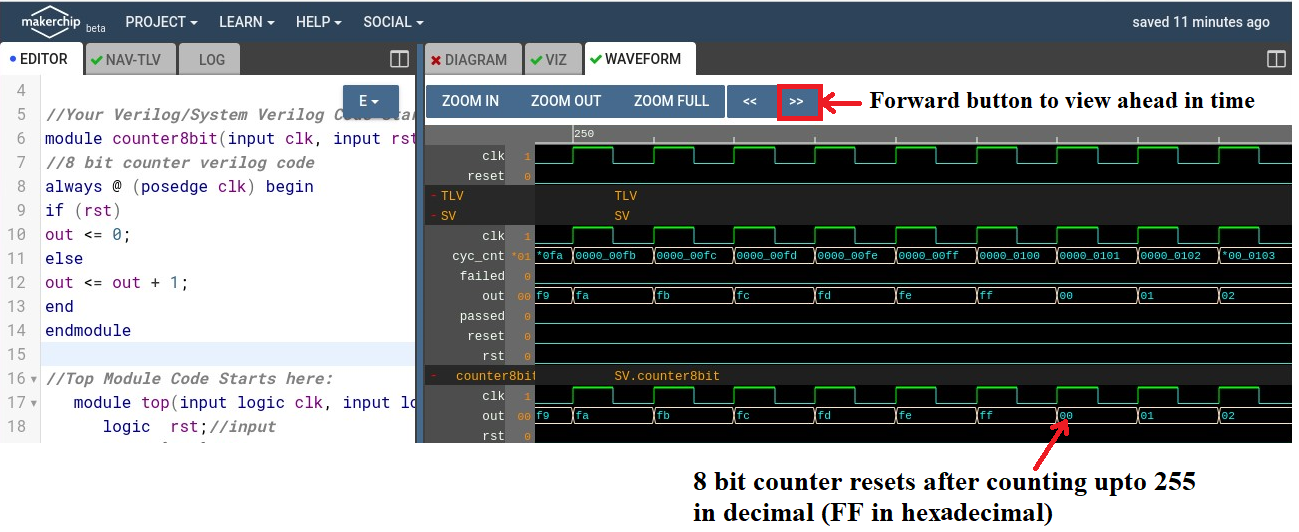
\includegraphics[width = 14cm, height =7cm]{./NgVeri/makerchipoutput3.png}
\caption{8 bit Counter counting from 0 to 255}
\label{output3}
\end{figure}

\item To view the output waveform forward in time, click on forward button as shown in \figref{output3}. It can be clearly seen, the 8 bit counter counts from to 0 to 255 in decimal (FF in hexadecimal) and it resets after counting up to 255. 

\item Next, close the Makerchip window. This completes the 8 bit counter verilog code compilation and verification process using Makerchip IDE. 

\end{enumerate}

\subsection {Steps to run NgVeri in eSim}

Steps for schematic creation and simulation using NgVeri in eSim are as follows: 

\begin{enumerate}
\item The verilog code named counter8bit.v is loaded in editor space of Makerchip tab as shown in \figref{addingv}.


\item Click on \textbf{NgVeri} button and then click on \textbf{Run Verilog to Ngspice converter} button as shown in \figref{ngclick}. This step will convert 8 bit counter's verilog file to Ngspice model. The commands that run in the NgVeri terminal leads to creation of Ngspice(XSPICE) model of 8 bit counter are mentioned in following steps. 

\begin{figure}[H]
\centering
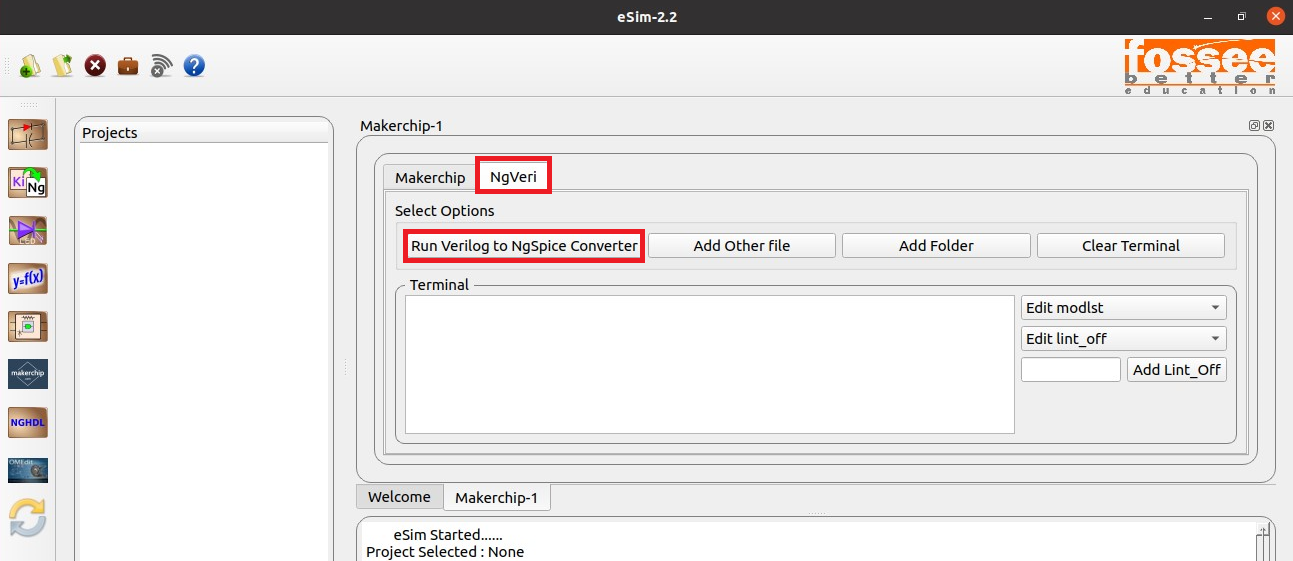
\includegraphics[width = 14cm, height =6cm]{./NgVeri/ngvericlick.png}
\caption{NgVeri interface buttons}
\label{ngclick}
\end{figure}

\item First command after clicking \textbf{Run Verilog to Ngspice Converter} button in NgVeri terminal is \textbf{RUN VERILATOR} highlighted as 1 in red color in \figref{ngvericommands}. 


\begin{figure}[H]
\centering
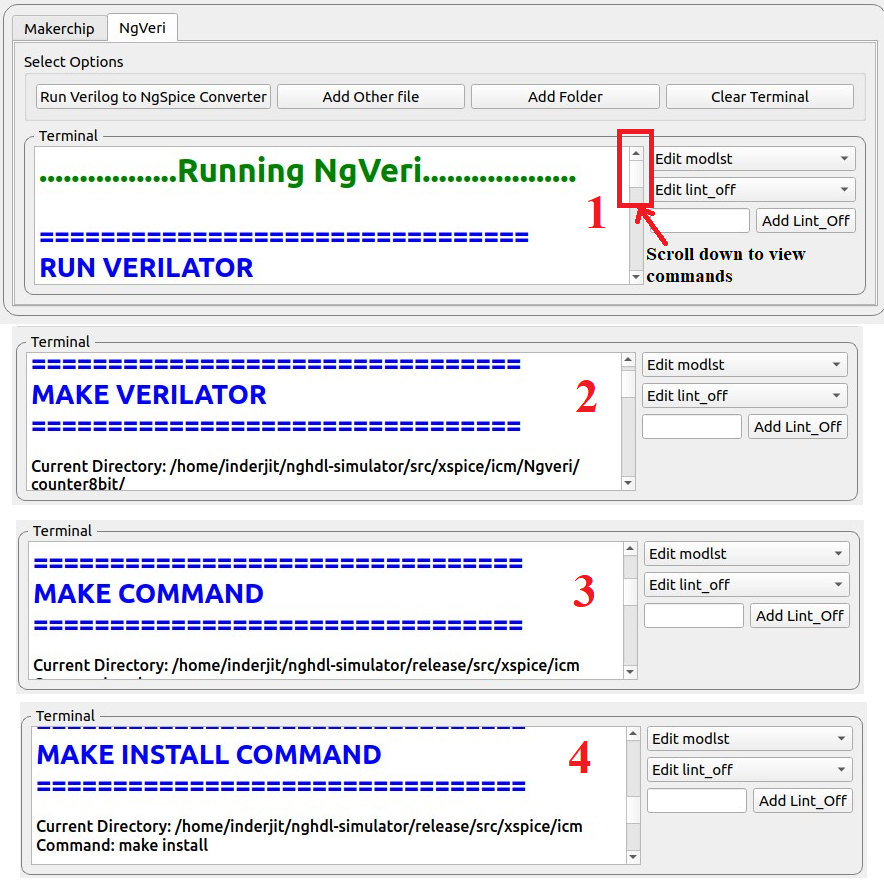
\includegraphics[width = 14cm, height =10cm]{./NgVeri/runverilator.png}
\caption{Commands in NgVeri}
\label{ngvericommands}
\end{figure}

\item Verilator converts the verilog file into C++ objects. Next command is\textbf{ MAKE VERILATOR} for obtaining the C++ objects. Next is \textbf{MAKE COMMAND}, which links the verilator's C++ objects and Ngspice objects.\textbf{ MAKE INSTALL COMMAND} is the last command in the process before Ngspice model creation.

\item When the \textbf{Model Created Successfully} message appears in the terminal as shown in green color in \figref{ngmodel}, it indicates that the Ngspice model is created.

\item An optional command \textbf{RUN SANDPIPER-SAAS} gets run Transaction-Level Verilog Code(.tlv) before the \textbf{RUN VERILATOR} command. This command in run to convert the Transaction-Level Verilog Code to the SystemVerilog Code which is easily accessible to the verilator.
\begin{figure}[H]
\centering
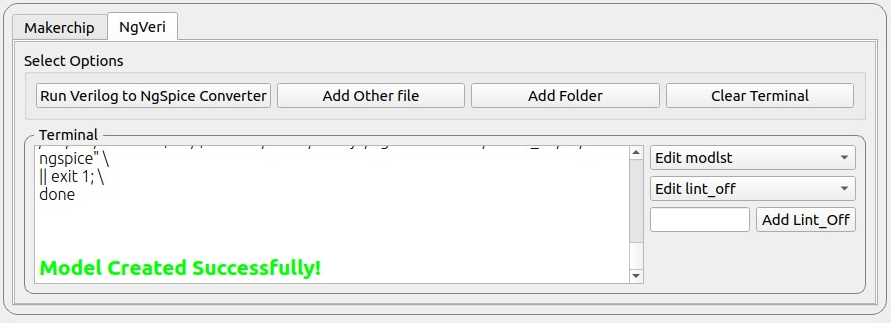
\includegraphics[width = 14cm, height =5cm]{./NgVeri/modelcreated.png}
\caption{NgVeri Model created}
\label{ngmodel}
\end{figure}



\begin{figure}[H]
\centering
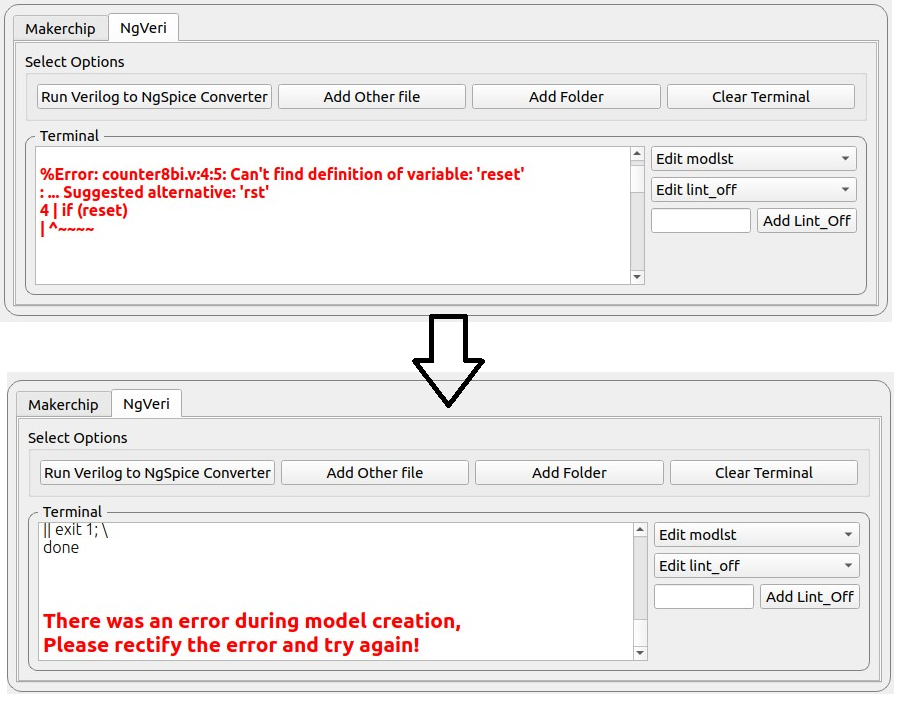
\includegraphics[width = 12cm, height =10cm]{./NgVeri/error1.png}
\caption{NgVeri Model creation error}
\label{ngverierror}
\end{figure}

\item In case of any error encountered in NgVeri terminal after running Verilog to Ngspice converter, then those errors will be displayed in the terminal in Red color in any of the commands discussed above. Debug the errors as per the messages displayed in the terminal. In \figref{ngverierror}, the error message is displayed in Red color in NgVeri terminal. 

\end{enumerate}

\subsection {Creating of Schematic of 8 bit counter}

In this section, we will create a new project in eSim, create the schematic and run the simulation for 8 bit counter. Steps for schematic creation are as follows:

\begin{enumerate}

\item Click on \textbf{New Project} icon to create a new project as shown in \figref{newproject}, be careful of the naming conventions.

\item After successful creation of NgVeri model using the Verilog code, you can create the schematic of your design by clicking on \textbf{Open Schematic} button on the left pane of the eSim window as shown in \figref{newschematic}. A confirmation pop-up window appears. Click on \textbf{Yes} to create a new schematic. A blank schematic created is shown in \figref{blankschematic}

\begin{figure}[H]
\centering
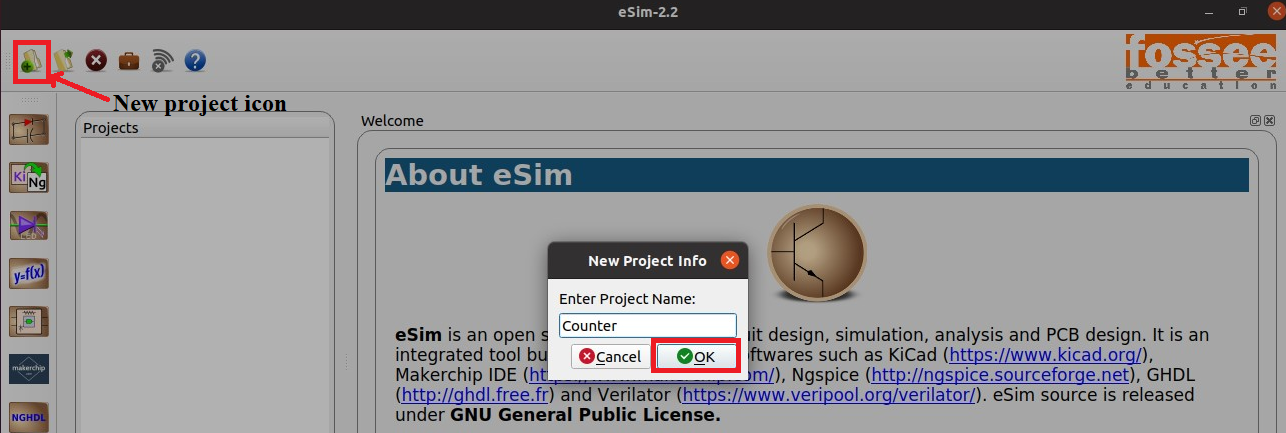
\includegraphics[width = 14cm, height =5cm]{./NgVeri/newproject.png}
\caption{Creation of new project in eSim}
\label{newproject}
\end{figure}

\item Next step is to click on \textbf{Place component} icon to place the components in the schematic editor as shown in \figref{blankschematic}.

\begin{figure}[H]
\centering
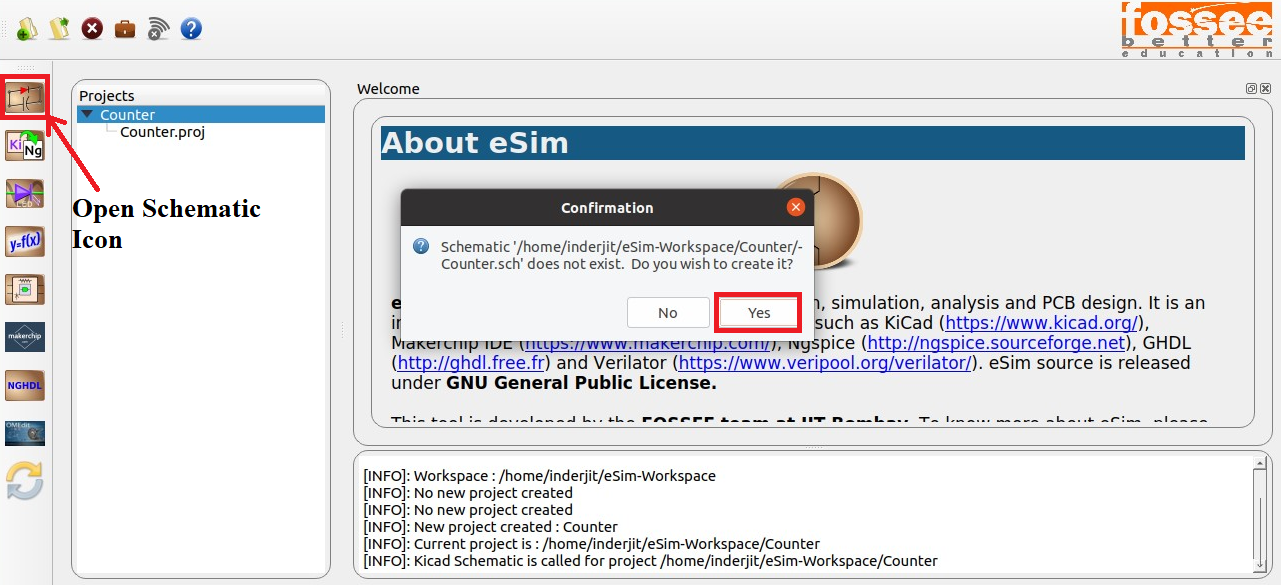
\includegraphics[width = 14cm, height =7cm]{./NgVeri/newschematic.png}
\caption{Creation of new schematic in eSim}
\label{newschematic}
\end{figure}

\begin{figure}[H]
\centering
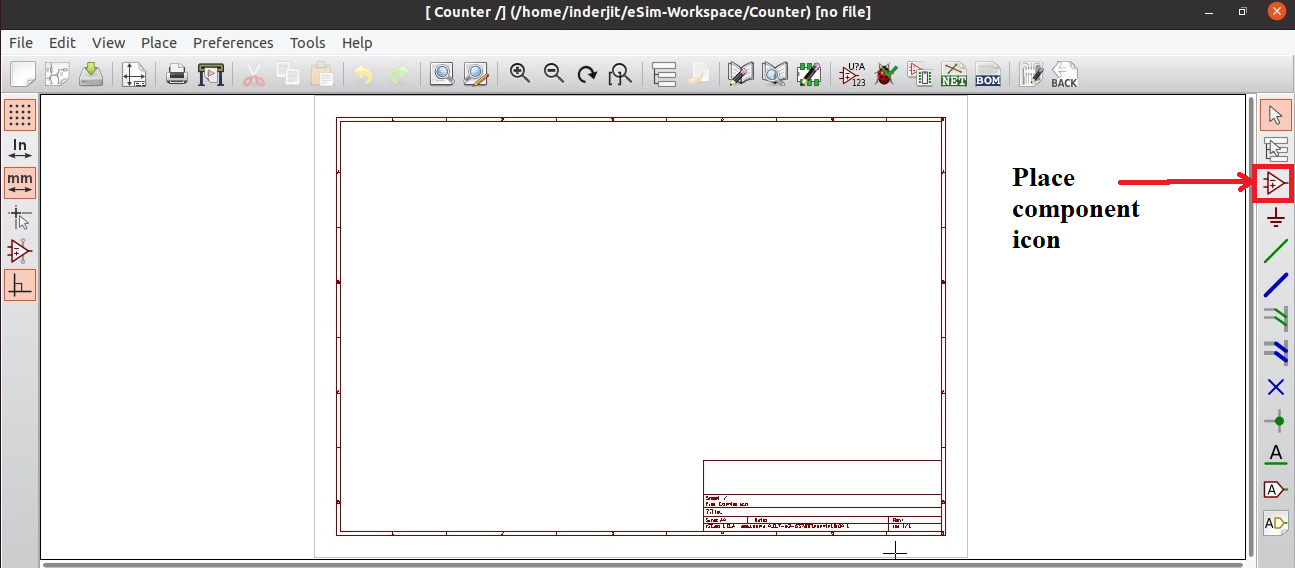
\includegraphics[width = 14cm, height =7cm]{./NgVeri/blankschematic.png}
\caption{Blank schematic created in eSim}
\label{blankschematic}
\end{figure}

\item To locate the components in eSim library, click on \textbf{Place component} icon as shown in \figref{blankschematic}. A pop-up window named \textbf{Choose Component} appears. User can type component name in the space as shown in \figref{choosemodel}. 

\begin{figure}[H]
\centering
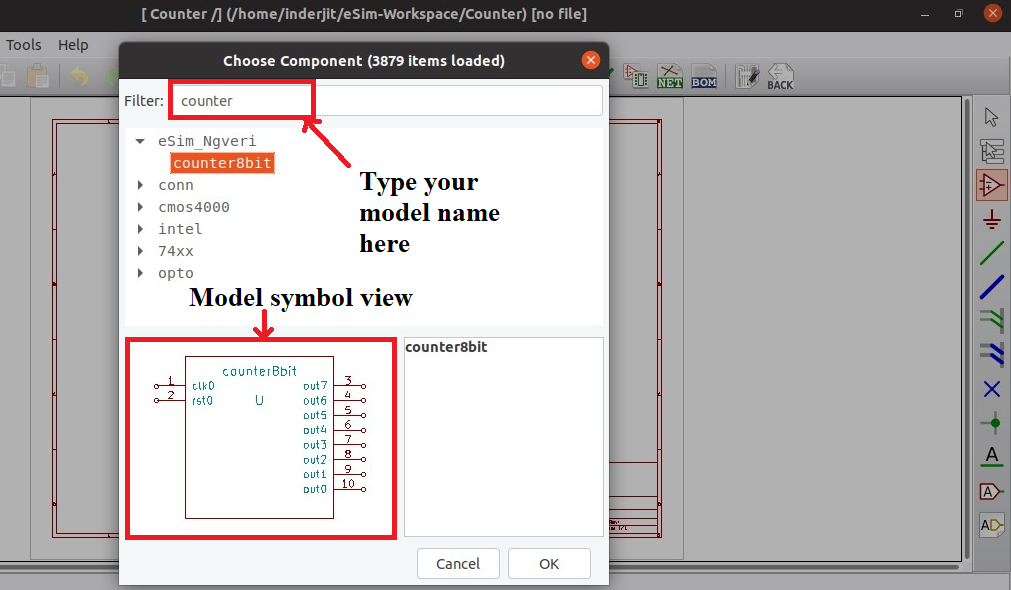
\includegraphics[width = 12cm, height =7cm]{./NgVeri/choosemodel.png}
\caption{Locating the model in library}
\label{choosemodel}
\end{figure}

\item In this example, counter8bit model is created under eSim NgVeri library. The model view is visible with two input pins reset and clock and 8 output pins from out0 to out7 as shown in \figref{choosemodel}. Click on \textbf{OK} to place the component on the schematic editor as shown in \figref{placemodel}.

\begin{figure}[H]
\centering
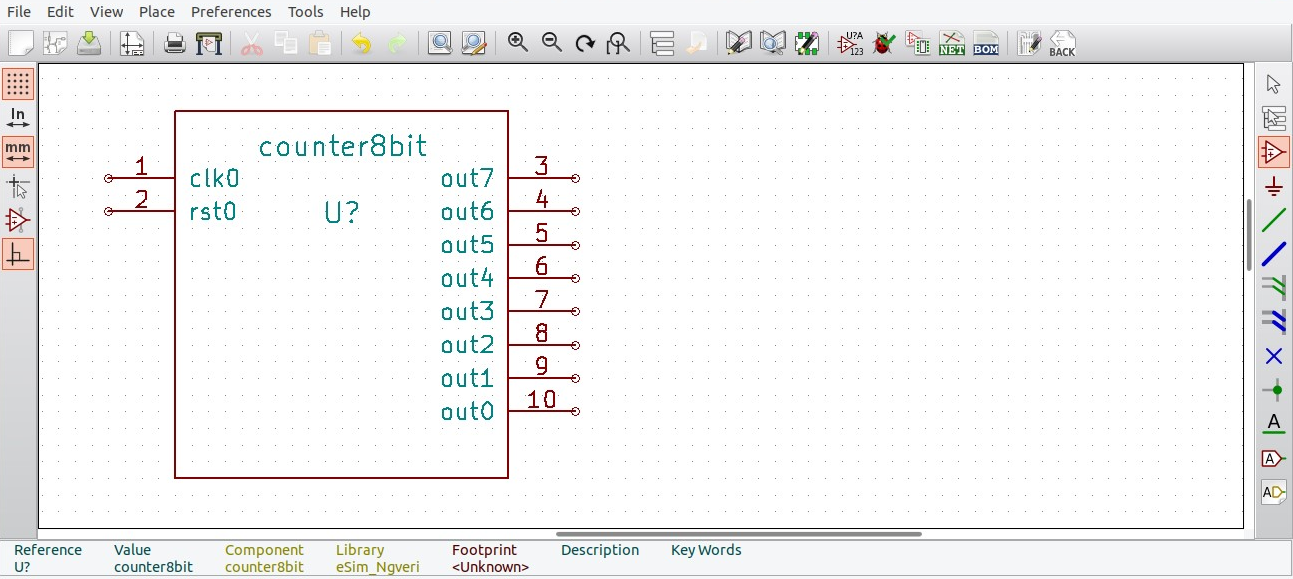
\includegraphics[width = 14cm, height =7cm]{./NgVeri/placingmodel.png}
\caption{Placement of component in Schematic Editor}
\label{placemodel}
\end{figure}

\item Now create the schematic as shown in \figref{circuitschematic}, annotate, perform electrical rules check (ERC), create the netlist and save the schematic by following the steps given in \chapref{chap5}.

\begin{figure}[H]
\centering
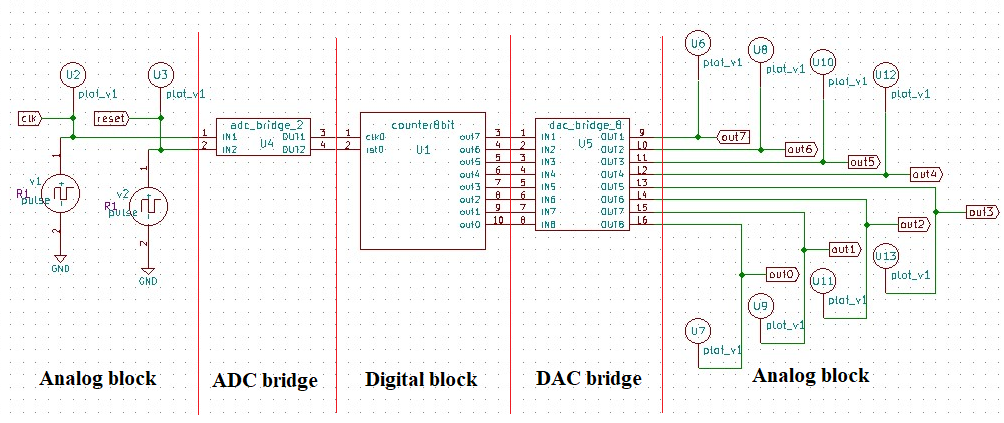
\includegraphics[width = 16cm, height =6cm]{./NgVeri/schematicwithblockdescription.png}
\caption{Example of a 8 bit Counter circuit in eSim}
\label{circuitschematic}
\end{figure}

\end{enumerate}

\subsection{Ngspice Simulation of 8 bit counter}

In this section, we will run the simulation and plot input-output waveforms for 8 bit counter. Steps for Ngspice simulation and plotting results are as follows:

\begin{enumerate}

\item After creating the schematic, click on \textbf{KiCad to Ngspice Converter} icon and select the type of analysis as transient and set the start, step and stop time as shown in \figref{kitong}

\begin{figure}[H]
\centering
\includegraphics[width = 14cm, height =6cm]{./NgVeri/KiCadtoNgspice.png}
\caption{KiCad to Ngspice conversion steps}
\label{kitong}
\end{figure}
 
 
\item Now click on Source Details and enter the values for Source v1 and Source v2 as shown in \figref{sourcev1} and \figref{sourcev2}

\begin{figure}[H]
\centering
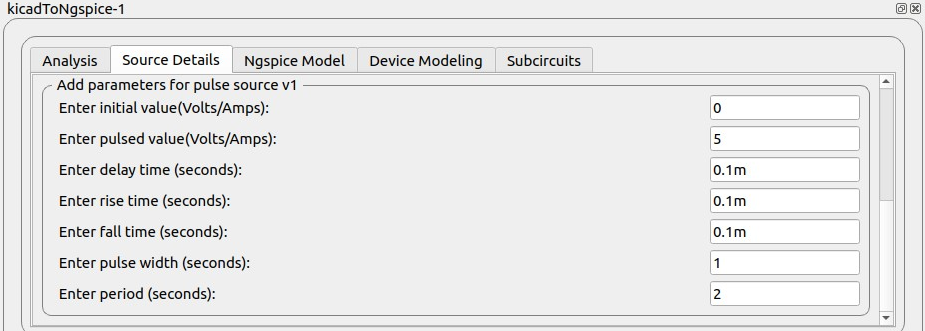
\includegraphics[width = 13cm, height =5cm]{./NgVeri/sourcev1.png}
\caption{Values for Source v1}
\label{sourcev1}
\end{figure}

\begin{figure}[H]
\centering
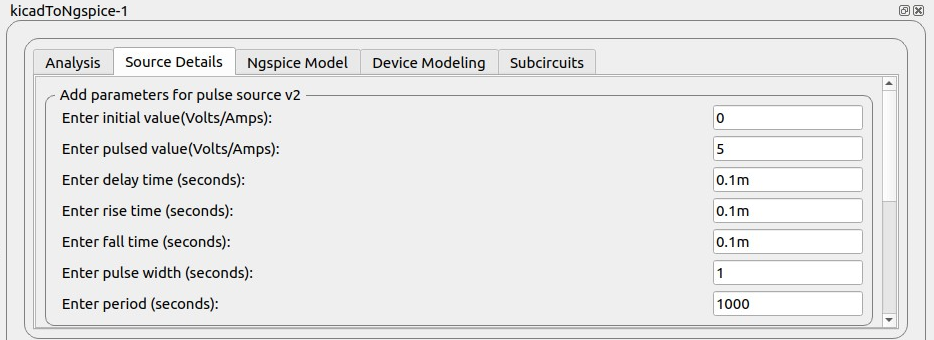
\includegraphics[width = 13cm, height =5cm]{./NgVeri/sourcev2.png}
\caption{Values for Source v2}
\label{sourcev2}
\end{figure}

\item In this counter example, no device modeling and sub-circuit build up is required. Now click on the \textbf{Convert} button as shown in \figref{KiCadconv}. This will convert KiCad schematic into Ngspice code i.e it creates the simulation compatible netlist.

\begin{figure}[H]
\centering
\includegraphics[width = 14cm, height =6cm]{./NgVeri/KiCadconv.png}
\caption{KiCad to Ngspice conversion}
\label{KiCadconv}
\end{figure}

\item Next, right click on \textbf{Counter} and click on \textbf{Refresh} as shown in \figref{refresh}. It can be seen that Project\_Name.cir.out file (Note: In this example, project name is Counter, so the file name is Counter.cir.out) is added after pressing refresh. Repeat this step for every rerun of KiCad to Ngspice conversion. 

\begin{figure}[H]
\centering
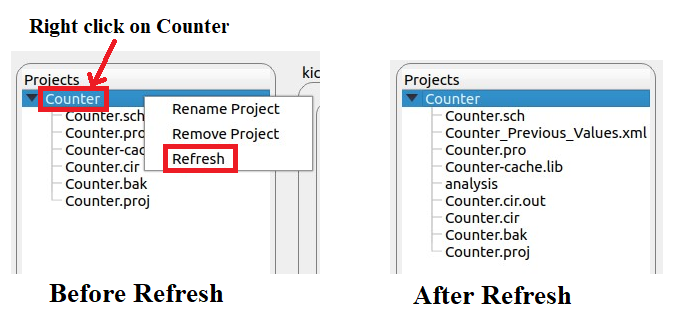
\includegraphics[width = 14cm, height =7cm]{./NgVeri/refreshbefore.png}
\caption{Cir.out file added after conversion}
\label{refresh}
\end{figure}

\item Next, right click on \textbf{Counter.cir.out} file and open it as shown in \figref{cirout1}. This file consists of Ngspice netlist of 8 bit counter including information of source, input and output plot labels, transient analysis parameters and control and plot statements. Refer \figref{cirout1} and \figref{cirout2}

\begin{figure}[H]
\centering
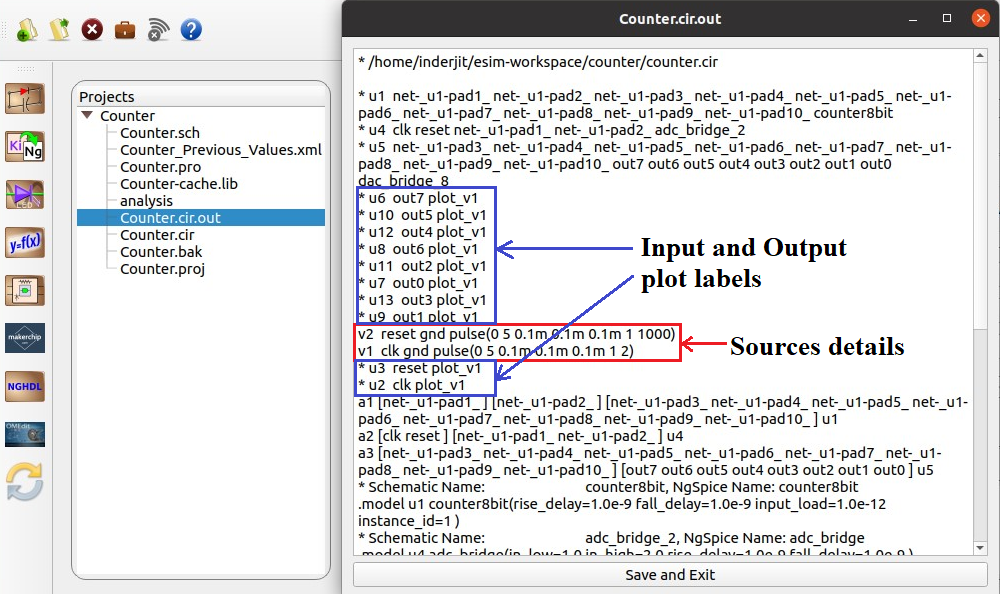
\includegraphics[width = 14cm, height =8cm]{./NgVeri/cirout1.png}
\caption{Cir.out file details Part 1}
\label{cirout1}
\end{figure}

\begin{figure}[H]
\centering
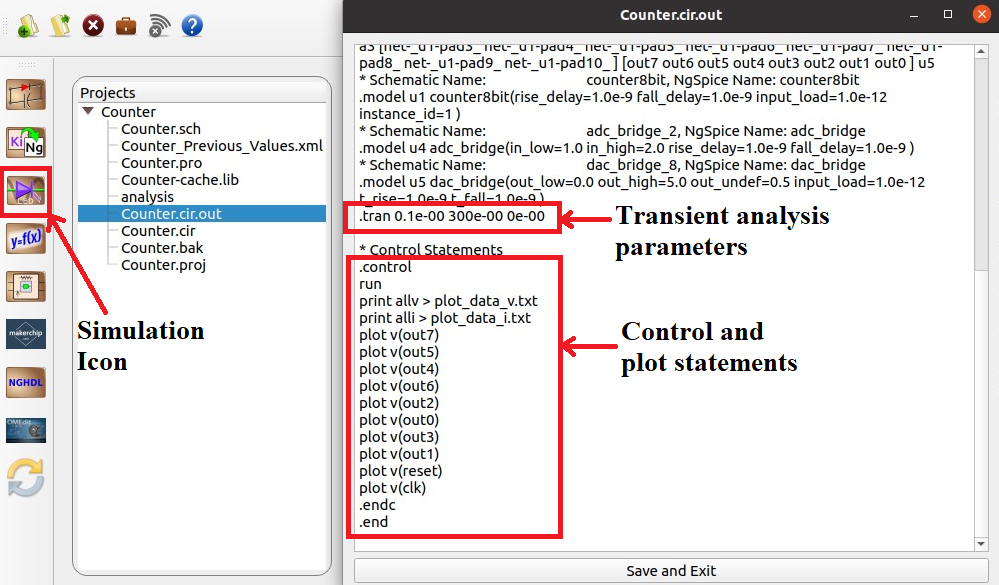
\includegraphics[width = 14cm, height =8cm]{./NgVeri/cirout2.png}
\caption{Cir.out file details Part 2}
\label{cirout2}
\end{figure}

\item To run simulation click on \textbf{Simulation} icon as shown in \figref{cirout2}. It will display input and output plots for 8 bit counter as shown in \figref{outputsim1}. You can see the plots of input clock, input reset and outputs out0 to out7. However, these plots are not in order. 

\begin{figure}[H]
\centering
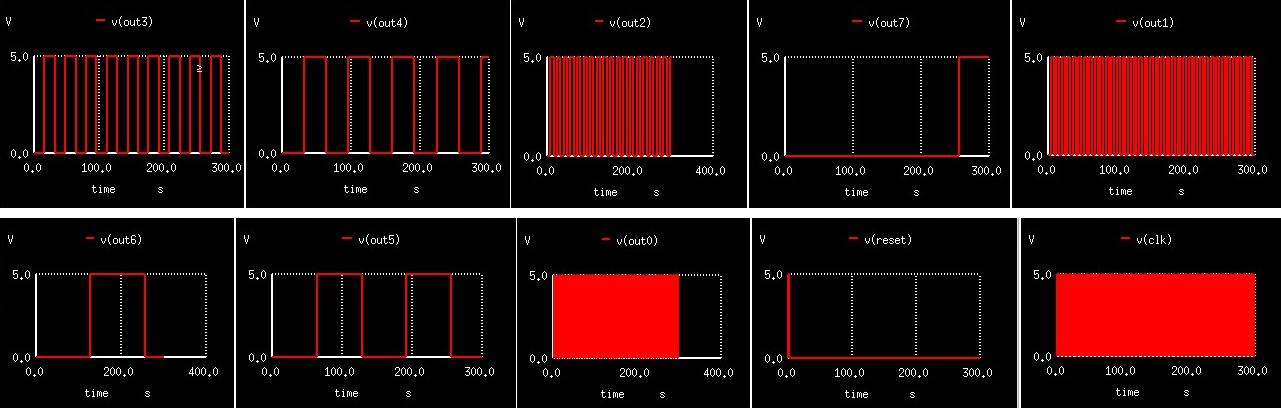
\includegraphics[width = 15cm, height =7cm]{./NgVeri/output1.png}
\caption{Input and Output simulation plots of 8 bit Counter}
\label{outputsim1}
\end{figure}

\item Close the simulations plots, and right click on \textbf{Counter} button and click on \textbf{Refresh} button as shown in \figref{refresh} to update the plot data files in the Projects folder. 

\begin{figure}[H]
\centering
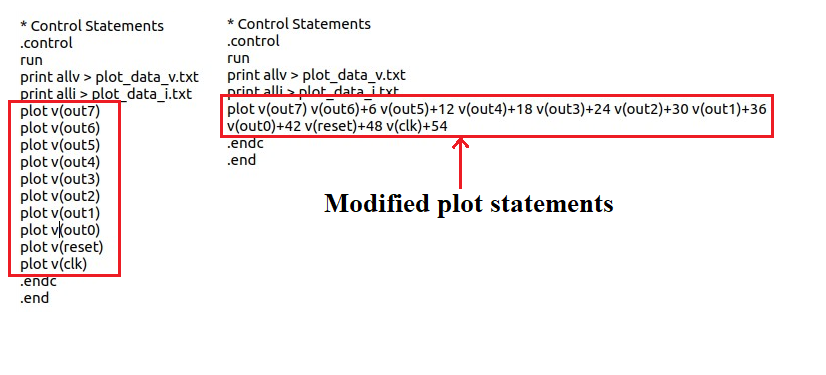
\includegraphics[width = 14cm, height =7cm]{./NgVeri/control1.png}
\caption{Editing the plots statements for stacked waveforms}
\label{control1}
\end{figure}


\begin{figure}[H]
\centering
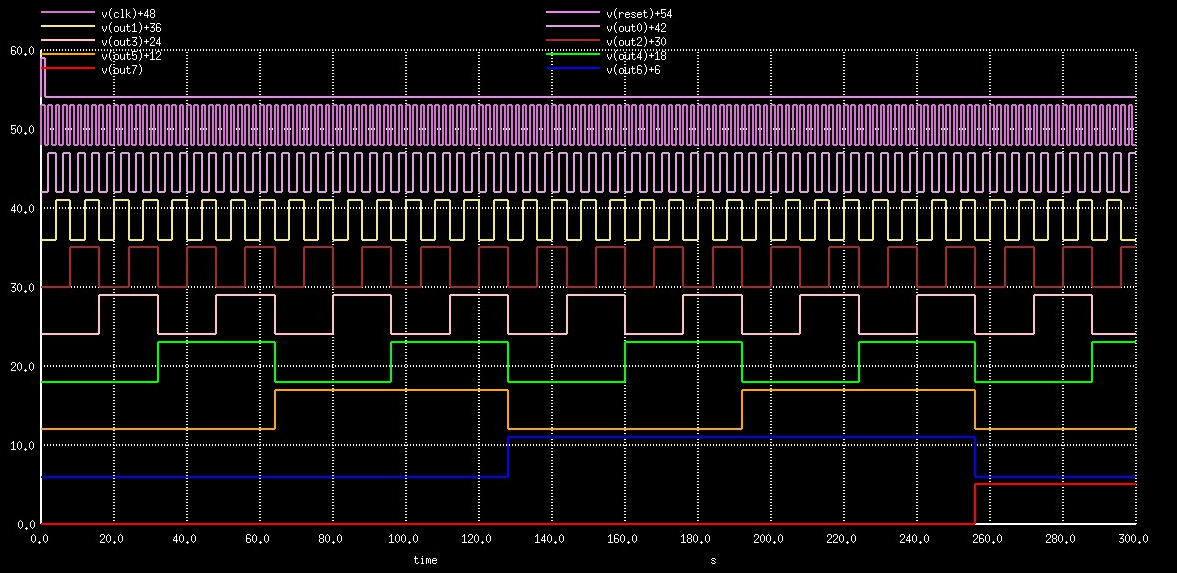
\includegraphics[width = 15cm, height =7cm]{./NgVeri/finalouput.png}
\caption{Stacked Input and Output Simulation plots of 8 bit counter}
\label{finaloutput}
\end{figure}

\item To view the plots in order and stacked manner, open Counter.cir.out file, do the changes in the plot statements as shown in \figref{control1}.

\item Running simulation again will result in the output of 8 bit counter as shown in \figref{finaloutput}. 

\end{enumerate}

\section {Common errors encountered in Makerchip-NgVeri:}

This section describes the most common errors faced by the user while building projects using Makerchip-NgVeri feature in eSim. 

\begin{enumerate}

\item In Makerchip tab, when the user clicks on Add Top Level Verilog button to load the file, the allowed file extension's should be either .v, .sv or .tlv as shown in \figref{filext}. It will not accept any other file extension. 

\begin{figure}[H]
\centering
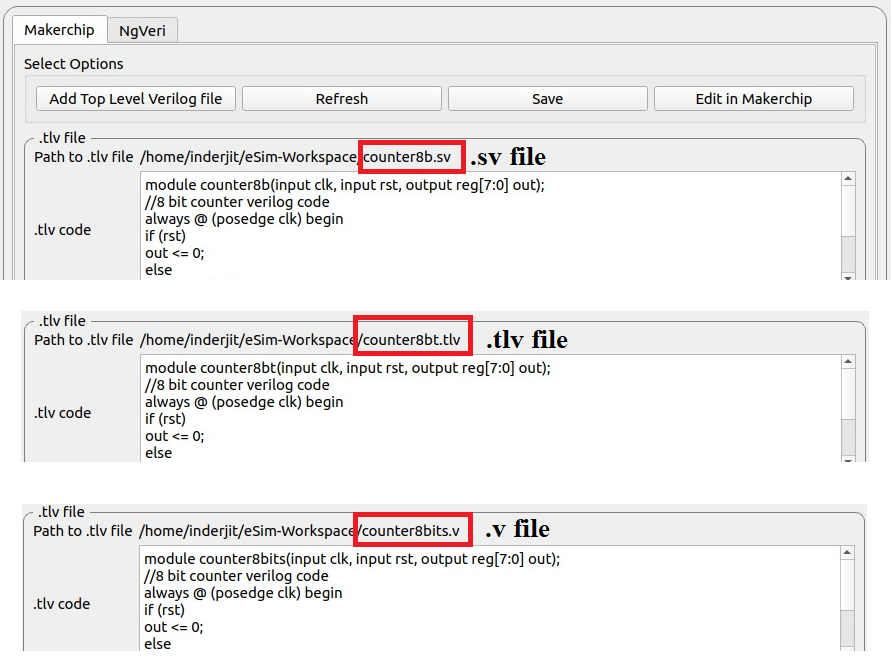
\includegraphics[width = 14cm, height =11cm]{./NgVeri/svfile.png}
\caption{File extension allowed in NgVeri}
\label{filext}
\end{figure}


\item User should avoid spaces or special characters in the path to file. \figref{path} shows file path and workspace path without any spaces and special characters. 


\begin{figure}[H]
\centering
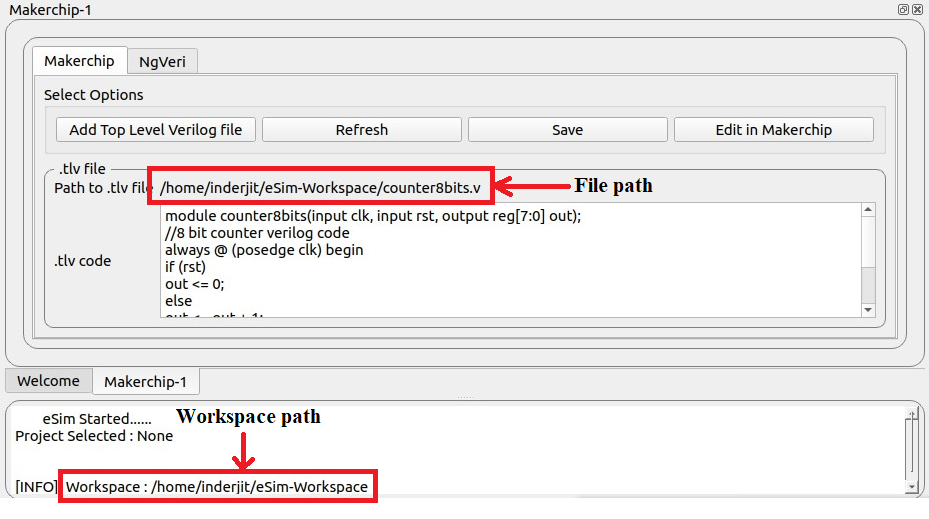
\includegraphics[width = 14cm, height =8cm]{./NgVeri/path.png}
\caption{File and workspace path without spaces and special characters}
\label{path}
\end{figure}

\item The verilog file should have Read and write Permissions. To set read and write permissions of the verilog file, right click on verilog file and click on \textbf{Properties}. Next click on \textbf{Permissions} and select access as \textbf{Read and write} as shown in \figref{rdwr}. 

\begin{figure}[H]
\centering
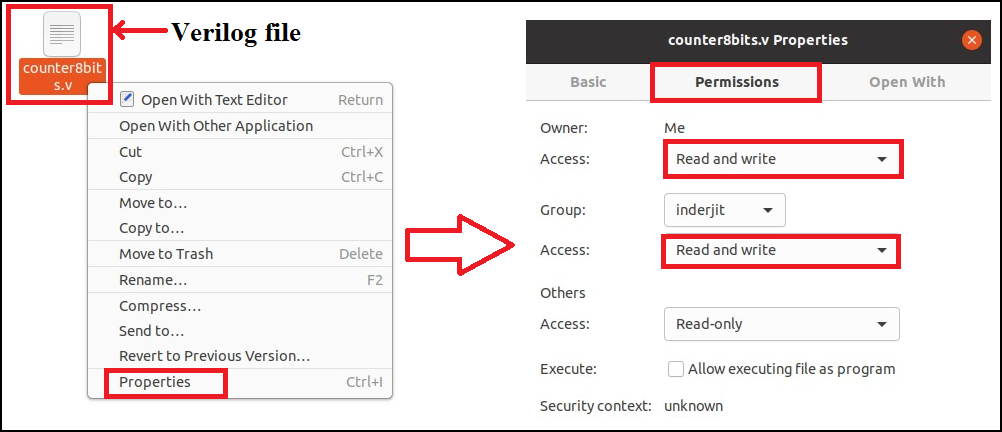
\includegraphics[width = 14cm, height =7cm]{./NgVeri/readwritepermission.png}
\caption{Read-Write Permissions for Verilog file}
\label{rdwr}
\end{figure}

\item Do not delete or rename the verilog file while it is loaded in eSim. 

\item If one gets an error in the NgVeri terminal, please clear the terminal and rerun. 

\item Do not use delays in the verilog code (as verilator does not support it). 

\item Verilog filename should be the same as top-level verilog module name, otherwise the following error message will appear as shown in \figref{error1}. This error appears when a user tries to open TL verilog in Makerchip by clicking \textbf{Edit in Makerchip} button.

\begin{figure}[H]
\centering
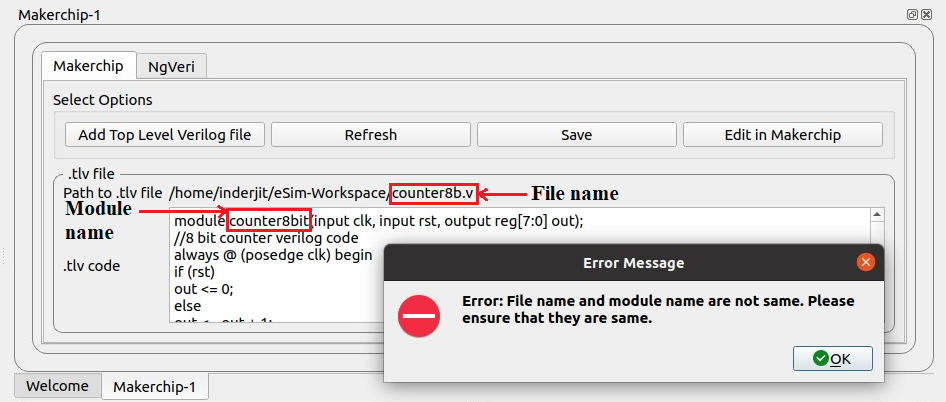
\includegraphics[width = 14cm, height =6cm]{./NgVeri/modulenameerror.png}
\caption{Verilog file and module name error}
\label{error1}
\end{figure}

\item \textbf{Verilator lint-off errors:} Lint-off commands will create this error in verilog code in Makerchip IDE can be resolved by removing such lint-off commands as shown in \figref{makerchiperror} and \figref{lintofferror}. Details about dealing with removal of such errors are already discussed in Makerchip steps in eSim. 

\item \textbf{Unexpected reg error:} This type of error can occur after compiling TL verilog code in Makerchip IDE visible in Log section (Refer \figref{regerror}). This error can be rectified by removing word \textit{reg} from top level verilog code as shown in \figref{removereg}. More details are discussed in Makerchip steps in eSim. 

\end{enumerate}



